%%%%%%%%%%%%%%%%%%%%%%%%%%%%%%%%%%%%%%%%%
% Beamer Presentation
% LaTeX Template
% Version 1.0 (10/11/12)
%
% This template has been downloaded from:
% http://www.LaTeXTemplates.com
%
% License:
% CC BY-NC-SA 3.0 (http://creativecommons.org/licenses/by-nc-sa/3.0/)
%
%%%%%%%%%%%%%%%%%%%%%%%%%%%%%%%%%%%%%%%%%

%----------------------------------------------------------------------------------------
%	PACKAGES AND THEMES
%----------------------------------------------------------------------------------------

\documentclass{beamer}

\mode<presentation> {

% The Beamer class comes with a number of default slide themes
% which change the colors and layouts of slides. Below this is a list
% of all the themes, uncomment each in turn to see what they look like.

%\usetheme{default}
%\usetheme{AnnArbor}
%\usetheme{Antibes}
%\usetheme{Bergen}
%\usetheme{Berkeley}
%\usetheme{Berlin}
%\usetheme{Boadilla}
%\usetheme{CambridgeUS}
%\usetheme{Copenhagen}
%\usetheme{Darmstadt}
%\usetheme{Dresden}
%\usetheme{Frankfurt}
%\usetheme{Goettingen}
%\usetheme{Hannover}
%\usetheme{Ilmenau}
%\usetheme{JuanLesPins}
%\usetheme{Luebeck}
\usetheme{Madrid}
%\usetheme{Malmoe}
%\usetheme{Marburg}
%\usetheme{Montpellier}
%\usetheme{PaloAlto}
%\usetheme{Pittsburgh}
%\usetheme{Rochester}
%\usetheme{Singapore}
%\usetheme{Szeged}
%\usetheme{Warsaw}

% As well as themes, the Beamer class has a number of color themes
% for any slide theme. Uncomment each of these in turn to see how it
% changes the colors of your current slide theme.

%\usecolortheme{albatross}
%\usecolortheme{beaver}
%\usecolortheme{beetle}
%\usecolortheme{crane}
%\usecolortheme{dolphin}
%\usecolortheme{dove}
%\usecolortheme{fly}
%\usecolortheme{lily}
%\usecolortheme{orchid}
%\usecolortheme{rose}
%\usecolortheme{seagull}
%\usecolortheme{seahorse}
%\usecolortheme{whale}
%\usecolortheme{wolverine}

%\setbeamertemplate{footline} % To remove the footer line in all slides uncomment this line
%\setbeamertemplate{footline}[page number] % To replace the footer line in all slides with a simple slide count uncomment this line

%\setbeamertemplate{navigation symbols}{} % To remove the navigation symbols from the bottom of all slides uncomment this line
}

\usepackage{graphicx} % Allows including images
\usepackage{booktabs} % Allows the use of \toprule, \midrule and \bottomrule in tables

%----------------------------------------------------------------------------------------
%	TITLE PAGE
%----------------------------------------------------------------------------------------

\title[Bayesian-Glasso Model]{Bayesian Glasso model for stock return series analysis} % The short title appears at the bottom of every slide, the full title is only on the title page
\author{Jian Wang } % Your name
\institute[Florida state university ] % Your institution as it will appear on the bottom of every slide, may be shorthand to save space
{Financial math Ph.D. candidate\\
\vspace{3ex}
Florida state university %%alifornia \\ % Your institution for the title page
\medskip
\textit{jwang@math.fsu.edu} % Your email address
}
\date{\today} % Date, can be changed to a custom date

\begin{document}

\begin{frame}
\titlepage % Print the title page as the first slide
\end{frame}

\begin{frame}
\frametitle{Overview} % Table of contents slide, comment this block out to remove it
\tableofcontents % Throughout your presentation, if you choose to use \section{} and \subsection{} commands, these will automatically be printed on this slide as an overview of your presentation
\end{frame}

%----------------------------------------------------------------------------------------
%	PRESENTATION SLIDES
%----------------------------------------------------------------------------------------

%------------------------------------------------
\section{Introduction} % Sections can be created in order to organize your presentation into discrete blocks, all sections and subsections are automatically printed in the table of contents as an overview of the talk
%------------------------------------------------

%\subsection{Subsection Example} % A subsection can be created just before a set of slides with a common theme to further break down your presentation into chunks

\begin{frame}
\frametitle{Introduction}
\begin{itemize}
\item Our final goal: Use efficient {\color{red}Bayesian} network to predict the stock return series
\item {\color{red}Lasso} model and {\color{red}Glasso} model for variable selection
\item Bayesian network structure learning based on the previous results of Glasso model
\item Model validation with famous bioinfo datasets
\item Pick one stock in the network and use {\color{red}linear regression},{\color{red} logistic regression} and {\color{red}{support vector machine}} to predict the future price
\item {\color{red}{Parallel computing}} and {\color{red}{high frequency data}}
\end{itemize}


\end{frame}

\section{Bayesian network}
\begin{frame}
\frametitle{Bayesian network}
\textbf{Bayesian network} is a probabilistic graphical model (a type of statistical model)
that represents a set of random variables and their conditional dependencies via a directed acyclic graph (DAG)\\
The following chart is an example of BN:\\
 \begin{figure}
     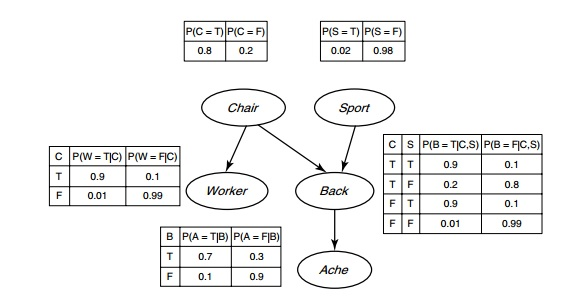
\includegraphics[width=0.9\textwidth]{bayesian.jpg}

    \end{figure}

\end{frame}


\begin{frame}
\frametitle{Bayesian network}

Three main research areas for Bayesian network\\
\begin{enumerate}
  \item {\color{red}Structure Learning}
  \item Parameter Learning
  \item Bayesian inference
\end{enumerate}

\end{frame}
\begin{frame}

\frametitle{Bayesian network}
Our main concern is on the structure learning process since it is exponentially increasing complicated and is the most challenging part in Bayesian network research area,here We aimed to use score based method to conduct the structure learning process.\\
\vspace{2ex}
BIC score:$BIC=-2*ln\hat{L}+K*ln(n)$, where:\\
\vspace{2ex}
$\hat{L}=$ maximum likelihood estimator, $k$ is the number of free parameters and $n$ is the number of data points in x
 \begin{figure}
     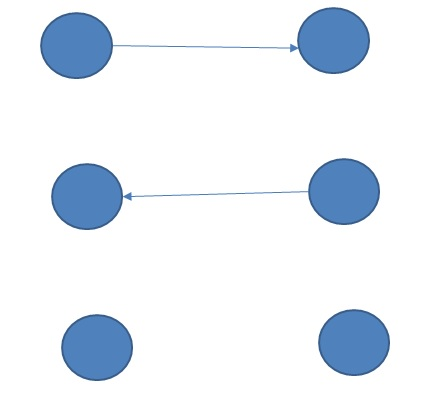
\includegraphics[width=0.4\textwidth, height=0.4\textheight]{learning.jpg}

    \end{figure}


\end{frame}

\section{Lasso and Glasso}

\begin{frame}
\frametitle{Lasso and Glasso }
Linear regression:$y_i = \beta_0+\sum_{j=1}^p{\beta_jx_{ij}}+\epsilon_i,  \epsilon_i$ i.i.d $\backsim N(0,\sigma^2) $
\setbeamercovered{transparent}
\begin{block}{Linear regression}
\begin{equation}
\hat{\beta}^{ls}=argmin_{\beta}\{\sum_{i=1}^p{(y_i-\hat{y_i})^2}\}
\end{equation}
\end{block}
\setbeamercovered{transparent}
\begin{block}{Ridge regression}
\begin{equation}
\hat{\beta}^{ridge}=argmin_{\beta}\{\sum_{i=1}^p{(y_i-\hat{y_i})^2}+{\color{red}\lambda \sum_{j=1}^p\beta_j^2}\}
\end{equation}
\end{block}

\begin{block}{Lasso regression}
\begin{equation}
\hat{\beta}^{lasso}=argmin_{\beta}\{\sum_{i=1}^p{(y_i-\hat{y_i})^2}+{\color{red}\lambda\sum_{j=1}^p \beta_j}\}
\end{equation}
\end{block}

\end{frame}


\begin{frame}
\frametitle{Lasso and Glasso }
Comparison of L1 and L2 Penalized Model \\
\begin{columns}
\column{2.3in}
	\begin{block}{Ridge regression}
$\hat{\beta}^{ridge}=argmin_{\beta}\{\sum_{i=1}^p{(y_i-\hat{y_i})^2}+{\color{red}\lambda \sum_{j=1}^p\beta_j^2}\}$

\end{block}
\textbf{Coefficients}:
 \begin{figure}
     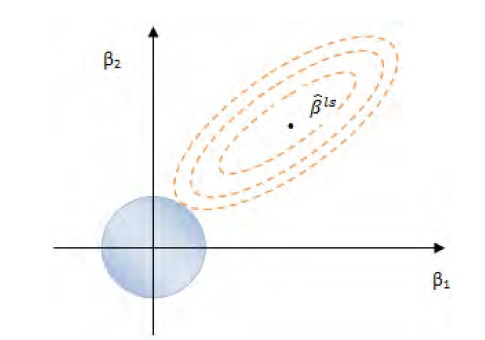
\includegraphics[width=0.9\textwidth, height=0.5\textheight]{ridge.jpg}

    \end{figure}

\column{2.3in}
\begin{block}{Lasso regression}

$\hat{\beta}^{lasso}=argmin_{\beta}\{\sum_{i=1}^p{(y_i-\hat{y_i})^2}+{\color{red}\lambda\sum_{j=1}^p \beta_j}\}$

\end{block}

\textbf{Coefficients}:
 \begin{figure}
     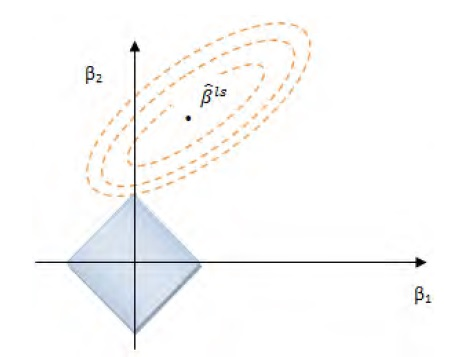
\includegraphics[width=0.9\textwidth, height=0.5\textheight]{lasso.jpg}

    \end{figure}
\end{columns}


\end{frame}

\begin{frame}
\frametitle{Lasso and Glasso }
Comparison of L1 and L2 Penalized Model \\
\begin{columns}
\column{2.3in}
	\begin{block}{Ridge regression}
$\hat{\beta}^{ridge}=argmin_{\beta}\{\sum_{i=1}^p{(y_i-\hat{y_i})^2}+{\color{red}\lambda \sum_{j=1}^p\beta_j^2}\}$

\end{block}
\textbf{Path:}:
 \begin{figure}
     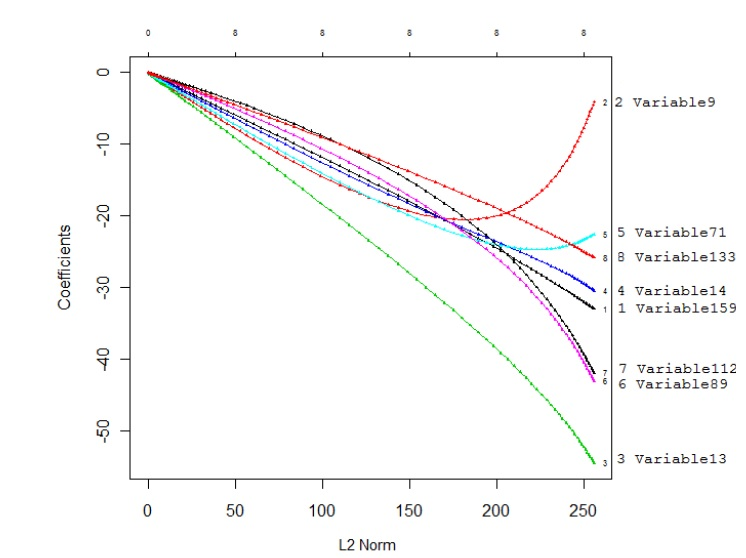
\includegraphics[width=0.9\textwidth, height=0.5\textheight]{ridge_p.jpg}

    \end{figure}

\column{2.3in}

\begin{block}{Lasso regression}

$\hat{\beta}^{lasso}=argmin_{\beta}\{\sum_{i=1}^p{(y_i-\hat{y_i})^2}+{\color{red}\lambda\sum_{j=1}^p \beta_j}\}$

\end{block}

\textbf{Path:}:
 \begin{figure}
     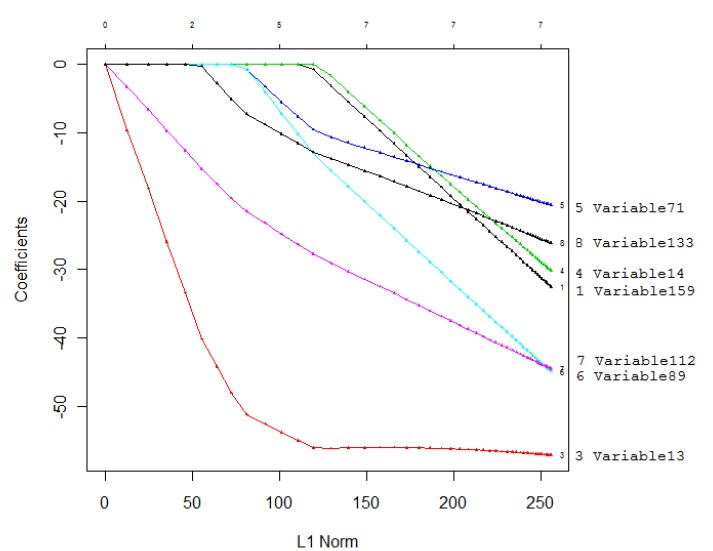
\includegraphics[width=0.9\textwidth, height=0.5\textheight]{lasso_p.jpg}

    \end{figure}
\end{columns}

\end{frame}

\begin{frame}
\frametitle{Lasso and Glasso }
  \setbeamercovered{transparent}
  \begin{block}{Reference:}
    \begin{itemize}
        \item  \textbf{The original paper:}\\
        Tibshirani, R. (1996). Regression shrinkage and selection via the lasso.
        \item  \textbf{The elast angle regression(LAR) algorithm for solving the Lasso:}\\
        Efron, B., Johnstone, I., Hastie, T. and Tibshirani, R. (2004). Least angle
       regression,
       \item  \textbf{Details and comparison:}\\
            Hastie, T., Tibshirani, R. and Jerome, F. The elements of statistical
            learning
    \end{itemize}
  \end{block}

  \begin{block}<2>{R packages}
    \begin{itemize}
        \item  LASSO in R: glmnet, lasso2, lars
        \item  Relaxed LASSO in R: relaxo
    \end{itemize}
  \end{block}

\end{frame}


\begin{frame}
\frametitle{Lasso and Glasso }
  \setbeamercovered{transparent}
  \begin{block}{Glasso:}
    Algorithm for learning the structure in an undirected Gaussian graphical model via using the $L_1$ regularization to control the
    zeros in the inverse covariance matrix\\
    Suppose we have N multivariate normal observations of dimension p , with mean $\mu$ and covariacne $\Sigma$. Let $\Theta=\Sigma^{-1}$ and $S$ be the empirical covariance matrix, the problem is to maximize the log- likelihood \\
    \begin{center}
    $logdet\Theta- tr(S\Theta))-\lambda||\Theta||_1$
  \end{center}
  \end{block}

  \begin{block}<2>{Algorithm}
  Many algorithms for this problem, The following might be the oldest and simple one by Meinshausen and Buhlmann(2006)
    \begin{itemize}
        \item  Estimate a sparse graphical model by fitting a lasso model to each variable, using others as predictors
        \item  Set $\Sigma_{ij}^{-1}$ to be non zero, if either the estimated coefficient of variable i on j, or the
        estimated coefficient of variable j on i, is non-zero
    \end{itemize}
  \end{block}
\end{frame}


\begin{frame}
\frametitle{Lasso and Glasso }
  \setbeamercovered{transparent}
  \begin{block}{Reference}
   \begin{itemize}
        \item Nicolai Meinshausen and Peter Buhlmann(2006),HIGH DIMENSIONAL GRAPHS AND VARIABLE SELECTION WITH THE LASSO
        \item Jerome Friedman,Trevor Hastie and Robert Tibshiraniz(2007), Sparse inverse covariance estimation with the graphical lasso
        \item Rahul Mazumder and Trevor Hastie,(2012),The graphical lasso: New insights and
alternatives

    \end{itemize}
  \end{block}

  \begin{block}<2>{R package}
    \begin{itemize}
        \item  Glasso: by Jerome Friedman, Trevor Hastie and Rob Tibshirani, from Standford, oldest one however updated till now(version 1.8)
        \item  Huge  by Tuo Zhao, Han Liu, Kathryn Roeder, John Lafferty, Larry Wasserman from John hopkins and CMU, developed by C instead of fortran, faster!

    \end{itemize}
  \end{block}

\end{frame}


\section{Bayesian-Glasso model}

\begin{frame}
\frametitle{Bayesian-Glasso model}
 For the high dimensional problem, it is not very easy to built the Bayesian network due to its exponentially increasing complexity. \\
 Our idea is to first use the Glasso model to conduct the model selection and then use Bayesian network structure learning process
 to define the network structure. \\
   \setbeamercovered{transparent}
   \begin{block}<2>{Algorithm}
    \begin{itemize}
        \item  Use Glasso algorithm to find the edges among variables
        \item  Use greedy search methods to change the direction only on those existed edges
        \item  Choose the direction which has the lowest BIC score
        \item  Finish when all the edges are reached or attain the maximum iteration numbers

    \end{itemize}
  \end{block}

\end{frame}

\begin{frame}
\frametitle{Bayesian-Glasso model}
One easy example(only contain three nodes) to illustrate the learning process as follows:\\
 \begin{center}
 \begin{figure}
     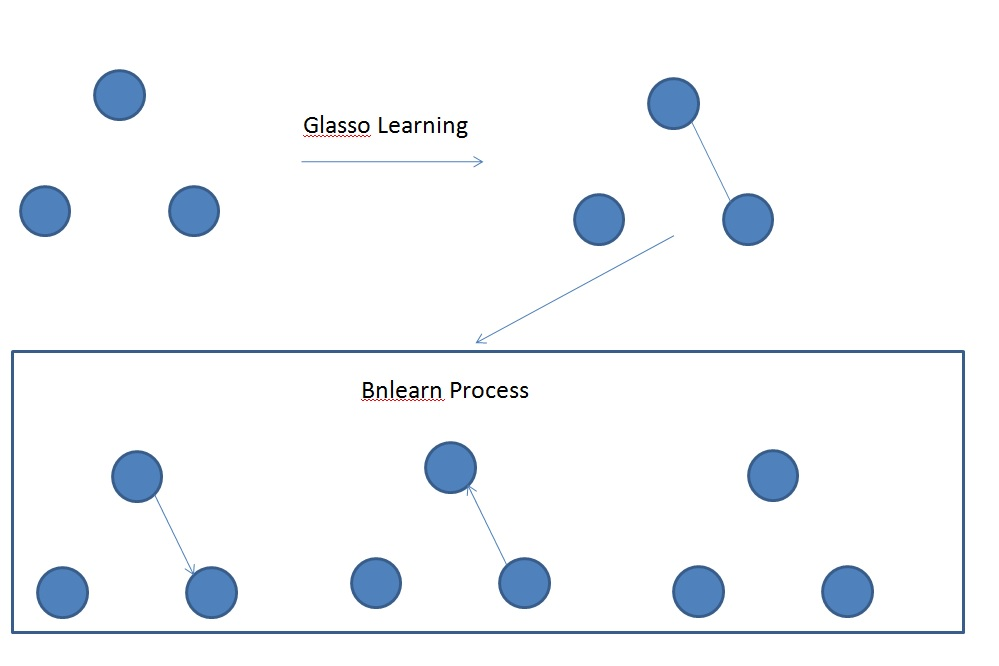
\includegraphics[width=0.8\textwidth, height=0.7\textheight]{bnglasso.jpg}

    \end{figure}
\end{center}

\end{frame}


\begin{frame}
\frametitle{Bayesian-Glasso model}
  \begin{block}{Famous data set test}
    \begin{itemize}
        \item  \textbf{ALARM}, with 37 nodes, 46 arcs and p=509 parameters
        \item  \textbf{HEPAR II}, with 70 nodes, 123 arcs and p = 1453 parameters
        \item  \textbf{ANDRES}, with 223 nodes, 338arcs and p = 1157 parameters
        \item  \textbf{PIGS} with 441 nodes, 592 arcs and 5618 parameters

    \end{itemize}
  \end{block}


\end{frame}

\begin{frame}
\frametitle{Bayesian-Glasso model}
  \begin{block}{ALARM}
  The left is the result of bayesnetwork model, the middle is the result of glasso model, the right is the result of Bayesian-Glasso model
 \begin{center}
 \begin{figure}
     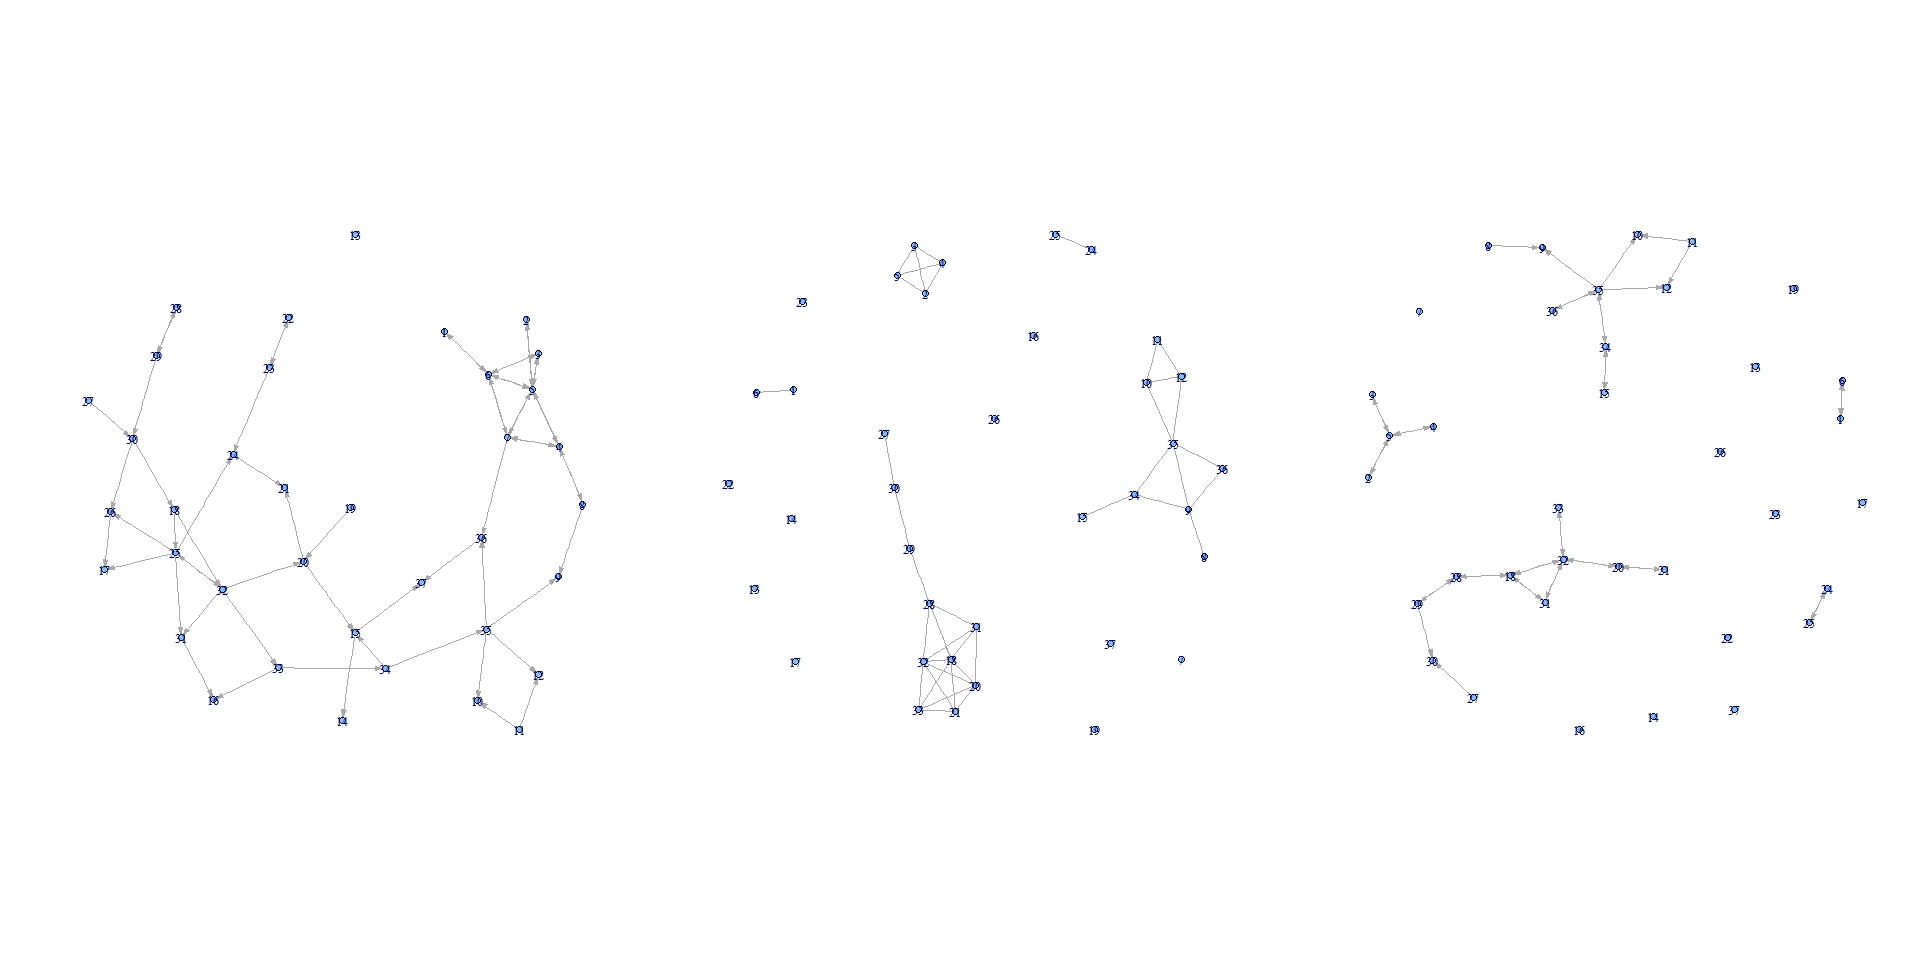
\includegraphics[width=0.9\textwidth, height=0.7\textheight]{alarm.jpeg}

    \end{figure}
\end{center}
  \end{block}


\end{frame}

\begin{frame}
\frametitle{Bayesian-Glasso model}
  \begin{block}{HEPARII}
  The left is the result of bayesnetwork model, the middle is the result of glasso model, the right is the result of Bayesian-Glasso model
 \begin{center}
 \begin{figure}
     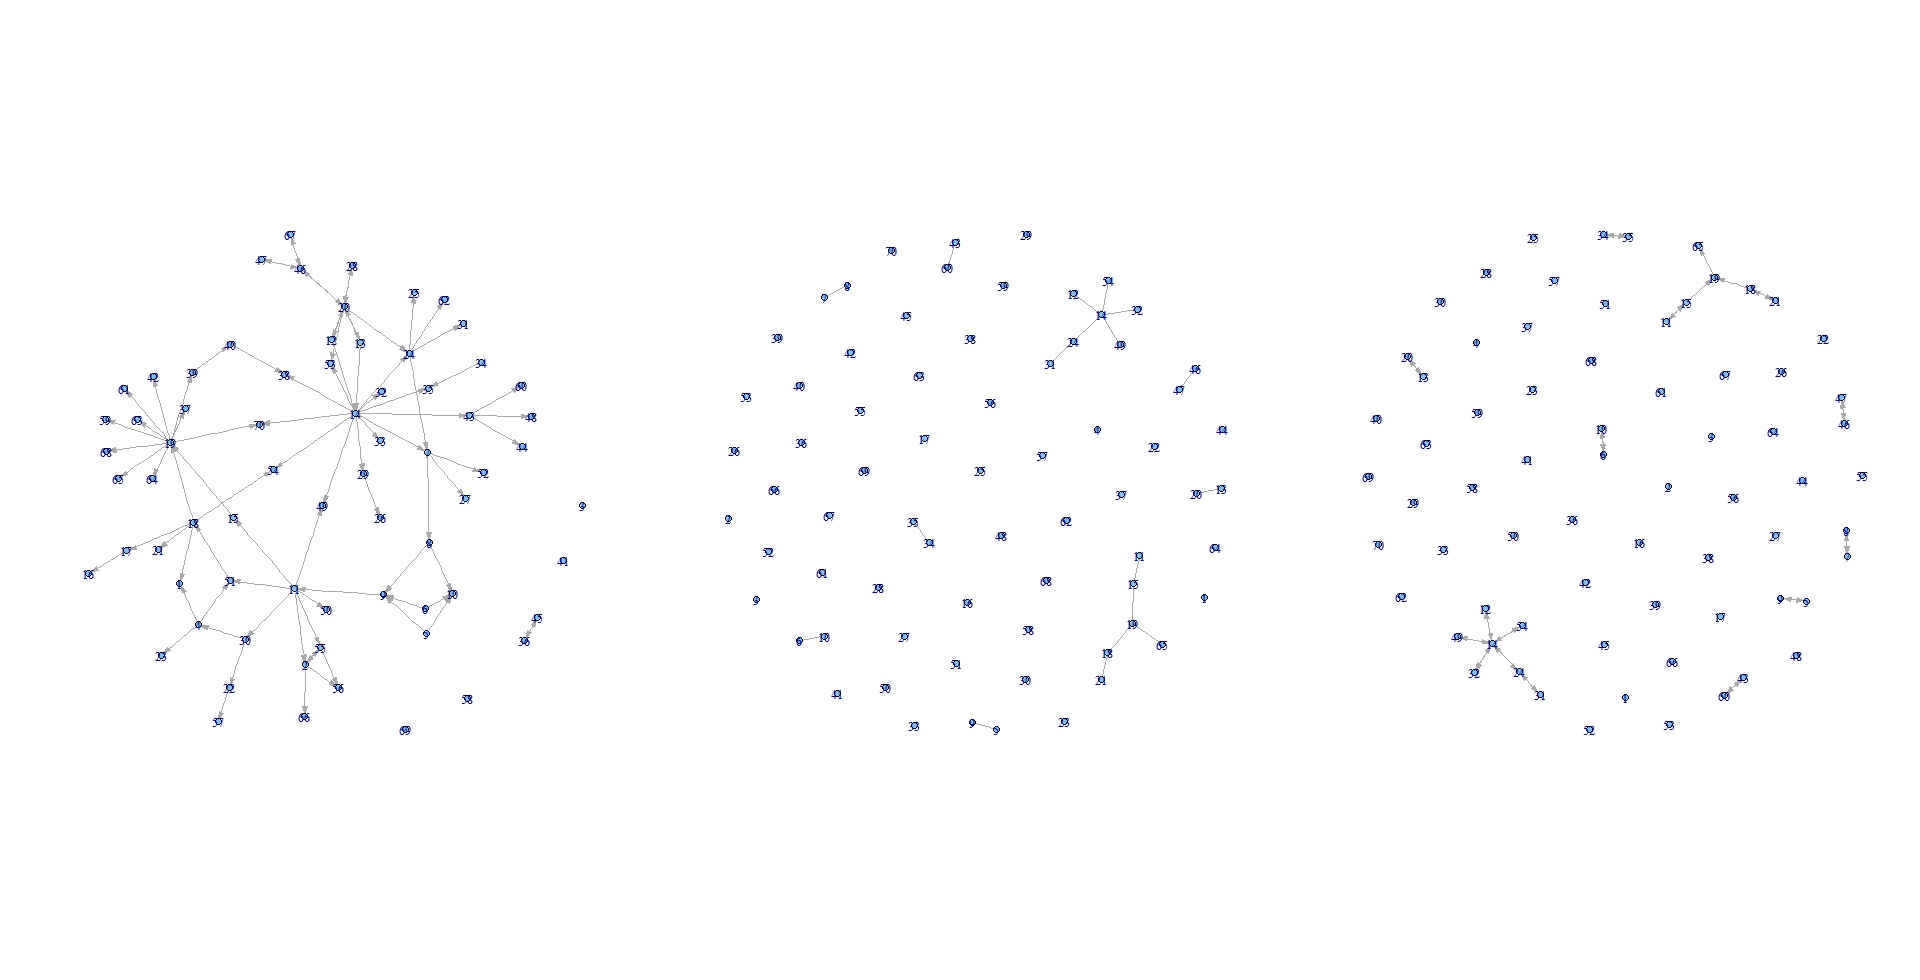
\includegraphics[width=0.9\textwidth, height=0.7\textheight]{hepar2.jpeg}

    \end{figure}
\end{center}
  \end{block}


\end{frame}

\begin{frame}
\frametitle{Bayesian-Glasso model}
  \begin{block}{ANDRES}
  The left is the result of bayesnetwork model, the middle is the result of glasso model, the right is the result of Bayesian-Glasso model
 \begin{center}
 \begin{figure}
     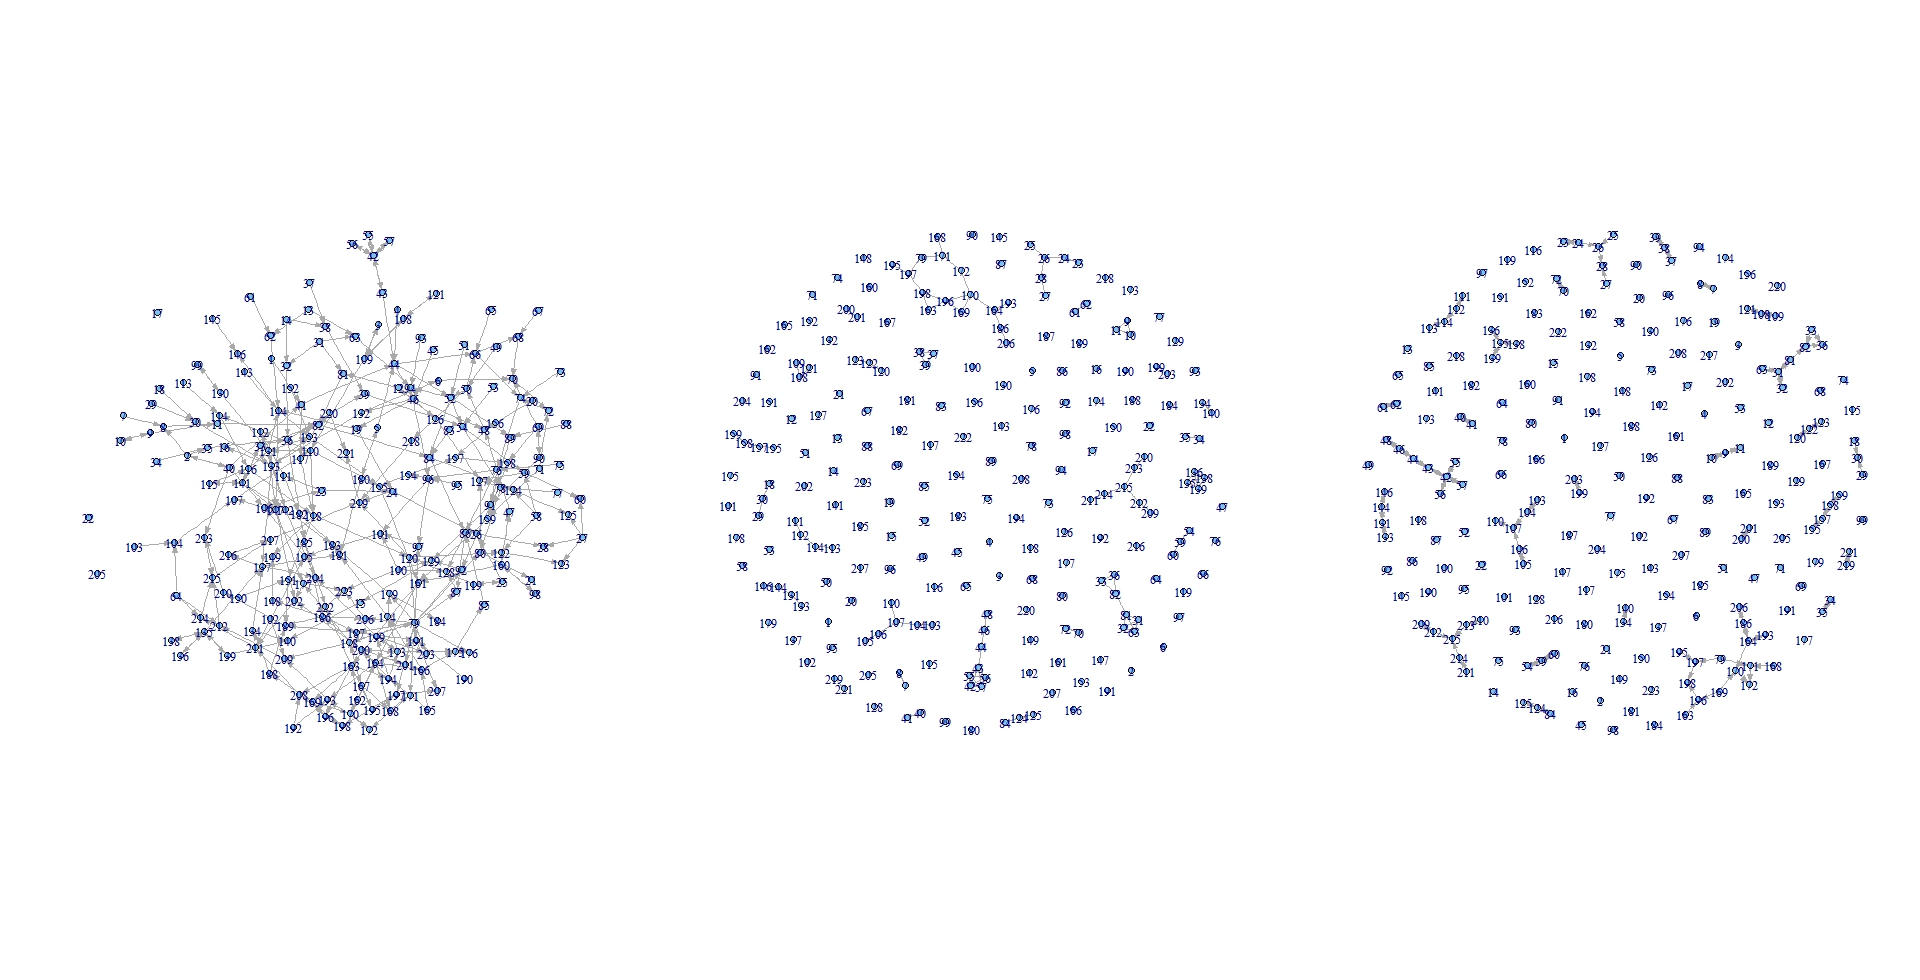
\includegraphics[width=0.9\textwidth, height=0.7\textheight]{andres.jpeg}

    \end{figure}
\end{center}
  \end{block}


\end{frame}
\begin{frame}
\frametitle{Bayesian-Glasso model}
  \begin{block}{PIGS}
  The left is the result of bayesnetwork model, the middle is the result of glasso model, the right is the result of Bayesian-Glasso model
 \begin{center}
 \begin{figure}
     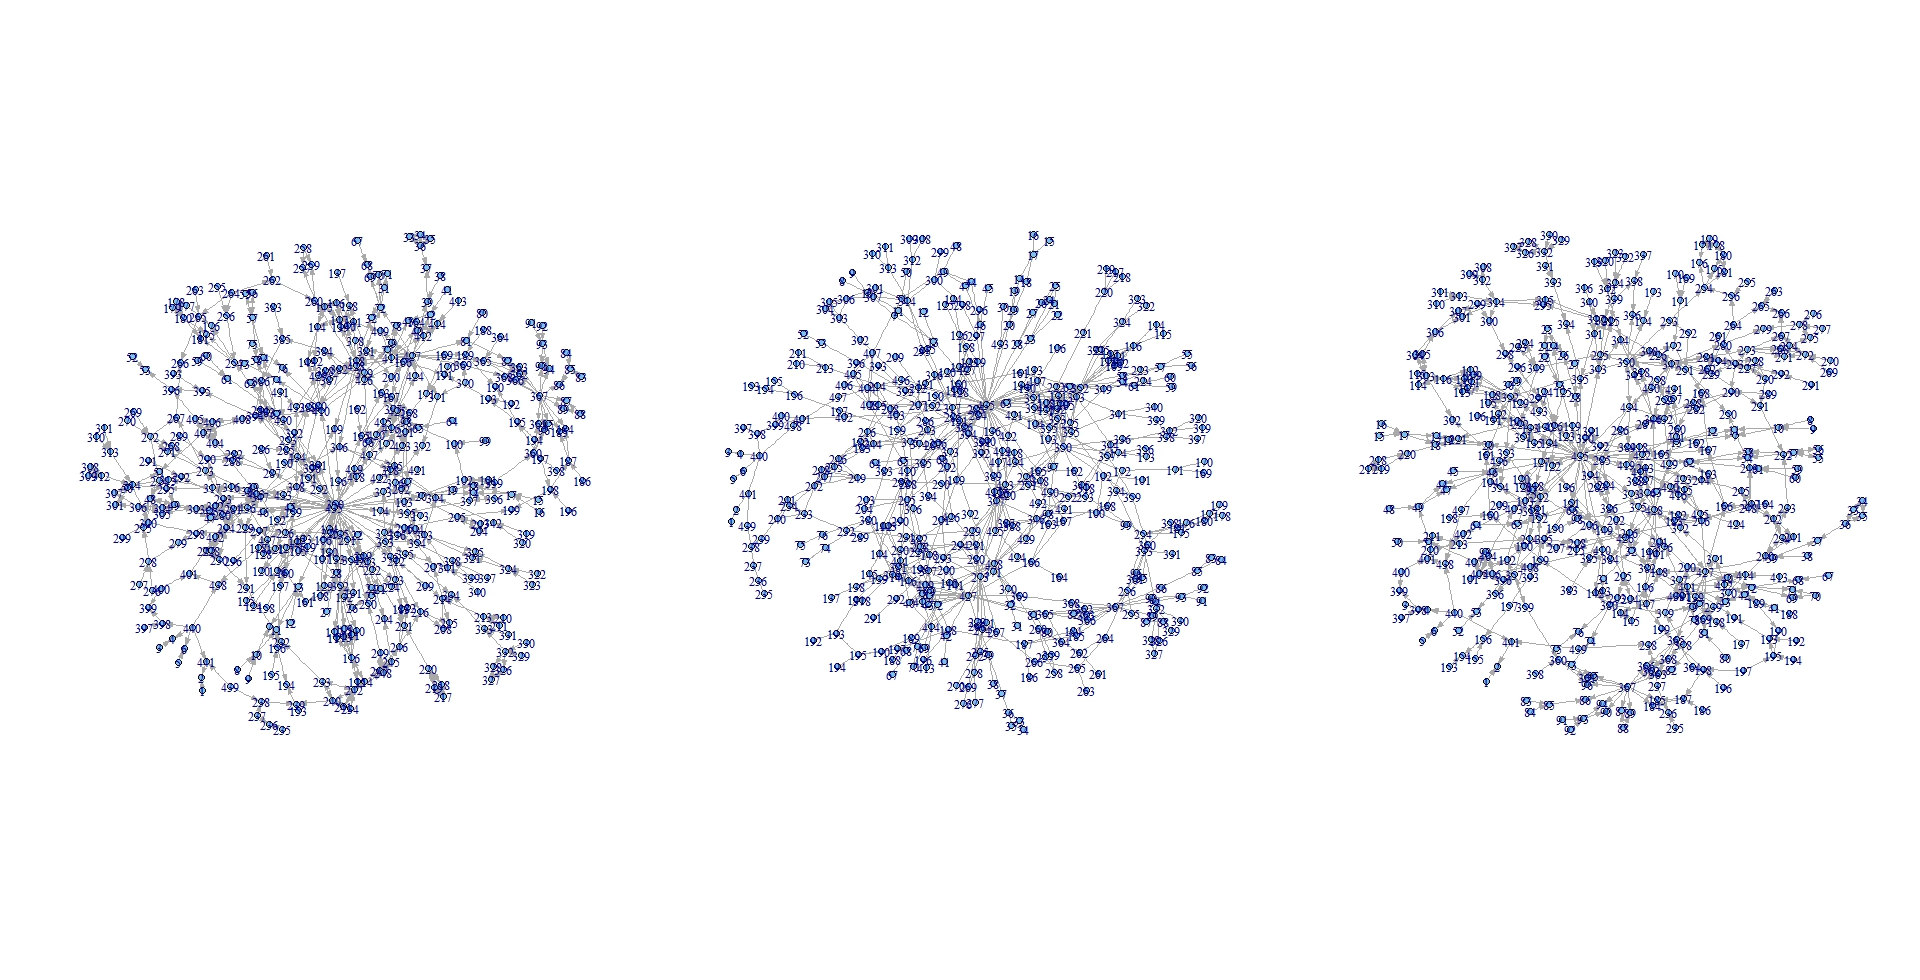
\includegraphics[width=0.9\textwidth, height=0.7\textheight]{pigs.jpeg}

    \end{figure}
\end{center}
  \end{block}


\end{frame}

\begin{frame}
\frametitle{Bayesian-Glasso model}
  \begin{block}{SCORE}
\begin{table}[h!]\large
  \caption{BIC scores for datasets}
\begin{center}
    \begin{tabular}{| c | c| c | }
    \hline
    Dataset& bn.hc &  bn.glasso\\
    \hline
ALARM &-54428&-69037\\
HEPARII&-163823&-167191\\
ANDES&-468395&-535242\\
PIGS &-1675890&-1684347\\
\hline
\end{tabular}
  \end{center}
\end{table}
\end{block}
  \begin{block}{Benefits}
    \begin{itemize}
        \item  The score function were all improved
        \item  The number of edges decreased

    \end{itemize}
  \end{block}

\end{frame}


\section {Stock data analysis}

\begin{frame}
\frametitle{Stock data analysis}
  \setbeamercovered{transparent}
\begin{block}{Data set}
\small{We chose the daily stock data set on the huge package, it contains the S\&P 500 stocks from the date January 1, 2003 to January 1, 2008. This gave us 1258 samples for the 452 stocks(reduced some stocks that are not during the entire period), Besides each stock was categorized into one industry and there are totally 10 industries according to the Global Industry Classification Standard(GICS),Use log return series of the stock for analysis}
\end{block}

\begin{block}<2>{Bayesian-Glasso learning results}
\begin{figure}
     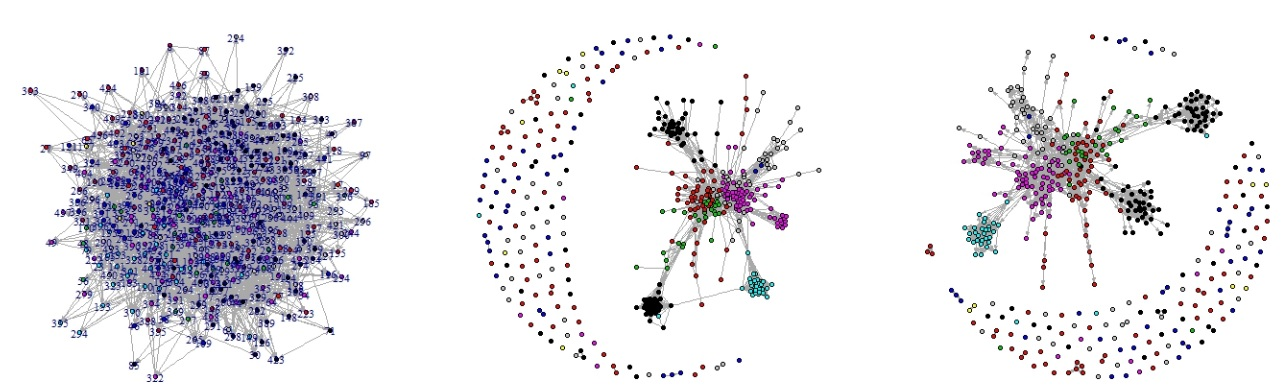
\includegraphics[width=0.9\textwidth, height=0.4\textheight]{stock.jpg}
    \end{figure}
\end{block}

\end{frame}

\begin{frame}

\begin{block}{Score}
\begin{table}[h!]\small
  \caption{BIC scores for Stockdata}
\begin{center}
    \begin{tabular}{| c | c| c | }
    \hline
    Dataset& bn.hc &  bn.glasso\\
    \hline
Stockdata &1543594&1510058\\
\hline
\end{tabular}
  \end{center}
\end{table}

\end{block}
\begin{block}{Forecast}
\small{Now random chose 1006 days without replacement as the training set and the remaining 251 days as the testing set.
We chose stock 186(GS),which had 7 parents, 15 (AA), 53 (BBT), 91(c),229(jpm),249(LNC),302(NTRS), 339(PFG)}\\
\begin{figure}
     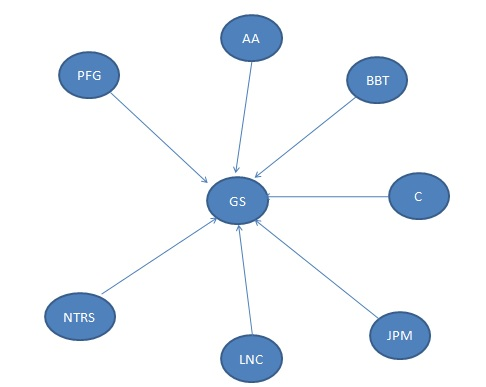
\includegraphics[width=0.5\textwidth, height=0.4\textheight]{gs.jpg}
    \end{figure}

\end{block}


\end{frame}

\begin{frame}

\begin{block}{Forecast}
Correlation and linear regression comparison:
\begin{figure}
     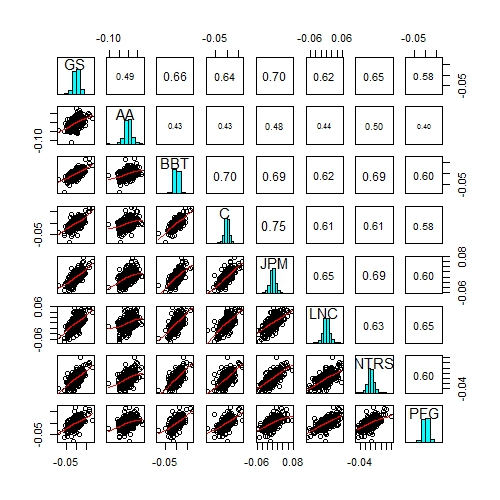
\includegraphics[width=0.8\textwidth, height=0.8\textheight]{gspairs.jpeg}
    \end{figure}

\end{block}


\end{frame}

\begin{frame}

\begin{block}{Forecast}

We classified the stock returns as increasing, unchanged and decreasing with the threshold 0.5\% and -0.5\%, to test the accuracy rate of the

model.

Among all the 251 days, there are 158 pairs between predicting values and true values that matched each other.

The accuracy rate for the model was around 63\% 


\end{block}

\end{frame}

\section{Future work}
\begin{frame}
\frametitle{Future work}
    \begin{itemize}
        \item  Compare with the time series model, such as Garch
        \begin{itemize}
        \item Stock return series is badly described by Gaussian(fat tailed and volatility cluster),most time series model assumed the normal or t distribution
        \item Only consider the stock itself, do not have some comprehensive-view
        \end{itemize}
        \item Parallel computing and high frequency data
        \begin{itemize}
        \item Multiple clusters, mpi and hadoop in software R
        \item How to deal with unsynchronized high frequency data
        \end{itemize}
      \end{itemize}


\end{frame}

%----------------------------------------------------------------------------------------

\end{document} 